% R008 — Guide to Cultivating Complex Analysis (Bahasa Indonesia)
% Reader-facing translation unit: source/ca-v1.9/ca.tex lines 1454–1537.
% Source release: v1.9 (commit a4d25d9ba37a486a5a020219eb8bd4e6602fd14c).
% Translation provenance: OpenAI Codex gpt-5.6-sol, Ultra, acting on the user's request.
% Preserve source equations, notation, references, labels, figure paths, and exercise states.

\section{Bola Riemann}

Kadang-kadang berguna untuk memperluas bilangan real dengan menambahkan $\pm \infty$.
Konsep serupa ada untuk bidang kompleks, meskipun
kita hanya menambahkan satu titik tak hingga.  Kita tulis
\glsadd{not:Cinfty}%
\glsadd{not:infty}%
\begin{equation*}
\C_{\infty} = \C \cup \{ \infty \} ,
\end{equation*}
dan kita menyebut $\C_{\infty}$ sebagai \emph{\myindex{bola Riemann}}.
Kita ingin topologi $\C_\infty$ sama dengan topologi $\C$
ketika kita berada jauh dari titik tak hingga.
Definisikan fungsi $g \colon \C_\infty \to \C_\infty$ dengan
\begin{equation*}
g(z) =
\begin{cases}
\nicefrac{1}{z} & \text{jika } z \neq 0 \text{ dan } z \neq \infty, \\
\infty & \text{jika } z = 0, \\
0 & \text{jika } z = \infty.
\end{cases}
\end{equation*}
Fungsi $g$ bersifat bijektif (satu-ke-satu dan surjektif).
Setiap lingkungan titik asal di $\C$ dipetakan ke suatu himpunan yang
memuat titik tak hingga, dan himpunan semacam itu kita sebut lingkungan
$\infty$.  Ketika membicarakan lingkungan
titik tak hingga di $\C_{\infty}$, sebenarnya kita ingin membayangkan pemetaan ini
dan lingkungan titik asal yang bersesuaian.

Secara lebih konkret, kita dapat memberikan struktur ruang metrik pada $\C_{\infty}$.
Misalkan $S^2$ adalah permukaan bola satuan di $\R^3$,
yaitu himpunan yang diberikan oleh $x^2 + y^2 + z^2 = 1$ bila $(x,y,z)$ adalah
koordinatnya.\footnote{Paragraf ini mungkin satu-satunya tempat dalam buku ini di mana
$z$ merupakan bilangan real.}  Bidang $\R^2$ dengan koordinat $(x,y)$ dapat
diidentifikasi dengan $\C$ berkoordinat $\xi$ dengan menetapkan $x+iy = \xi$.
Diberikan sembarang titik $p \in S^2$ yang bukan kutub utara $(0,0,1) \in S^2$,
terdapat tepat satu garis di $\R^3$ yang melalui titik $(0,0,1)$ dan $p$.
Tidak sulit membuktikan bahwa garis ini tidak pernah sejajar dengan
bidang $xy$, yaitu $\C$, sehingga garis tersebut harus memotong $\C$ di tepat satu
titik $\xi \in \C$ (sebuah bidang dan sebuah garis berpotongan di tepat satu titik kecuali
keduanya sejajar).  Definisikan
\begin{equation*}
\Phi(p) = \xi.
\end{equation*}
Tetapkan $\Phi\bigl((0,0,1)\bigr) = \infty$, sehingga kita memperoleh pemetaan
$\Phi \colon S^2 \to \C_\infty$.  Pemetaan ini disebut
\emph{\myindex{proyeksi stereografik}}.  Lihat
\figureref{fig:riemannsphere}.
Pemetaan ini bijektif (latihan di bawah),
sehingga kita dapat mendefinisikan metrik pada $\C_\infty$ dengan
menggunakan metrik pada $S^2$, yang dapat berupa metrik subruang
yang berasal dari metrik Euklides pada $\R^3$.
Kemungkinan lain
adalah jarak lingkaran besar, \exampleref{ms:greatcircle}.
Kedua jarak tersebut akan menghasilkan topologi yang sama, dan dengan demikian limit yang sama.

\begin{myfig}
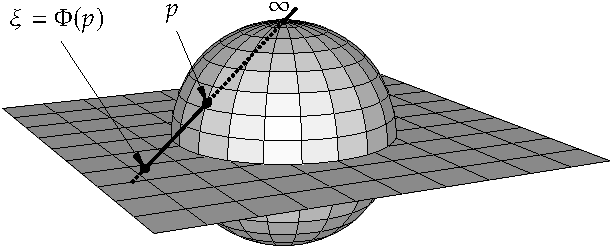
\includegraphics{figures/riemannsphere}
\caption{Proyeksi stereografik dari bola $S^2$ ke bidang
kompleks.\label{fig:riemannsphere}}
\end{myfig}

\begin{exbox}
\begin{exercise}%[\neededexmark]
Tunjukkan bahwa $\Phi$ bijektif.
\end{exercise}

\begin{exercise}
Misalkan $(\phi,\theta)$
adalah koordinat bola pada $S^2$, dengan $0 \leq \phi \leq \pi$ sebagai zenit (sudut yang dibentuk
dengan sumbu-$z$) dan $-\pi < \theta \leq \pi$ sebagai azimut, serta kita menuliskan
titik-titik di $\C$ menggunakan koordinat polar $re^{i\theta}$.  Buktikan bahwa
$\Phi$ memetakan
$(\phi,\theta)$ ke $\cot (\nicefrac{\phi}{2})\,e^{i\theta}$.
\end{exercise}

\begin{exercise}%[\neededexmark]
Tunjukkan bahwa topologi yang diinduksi pada $\C$ oleh topologi $S^2$ melalui $\Phi$
seperti di atas ekuivalen dengan topologi standar.  Artinya, tunjukkan bahwa himpunan $U
\subset \C$
terbuka dalam metrik Euklides pada $\C$ jika dan hanya jika terbuka menurut
metrik yang berasal dari $S^2$.
\end{exercise}
\end{exbox}
